Le graphe se construit en considérant chaque ville à différents moment : jeudi matin, jeudi soir, vendredi matin, vendredi soir, et samedi matin. F le samedi soir sera considéré comme le puits du graphe.

On note par ailleurs que le séjour dans une ville la journée n'est pas limité en quantité, on peut donc construire un arc entre une ville le matin et la même ville le soir avec une capacité infinie.

Sur le graphe de la figure~\ref{fig:pass:un}, chaque sommet est nommé à partir de 3 lettres : la première représente la ville (A,  B, C ou F), la seconde le jour (J, V, S) et la troisième le moment de la journée (M, S).

\begin{figure}[h]
\begin{center}
	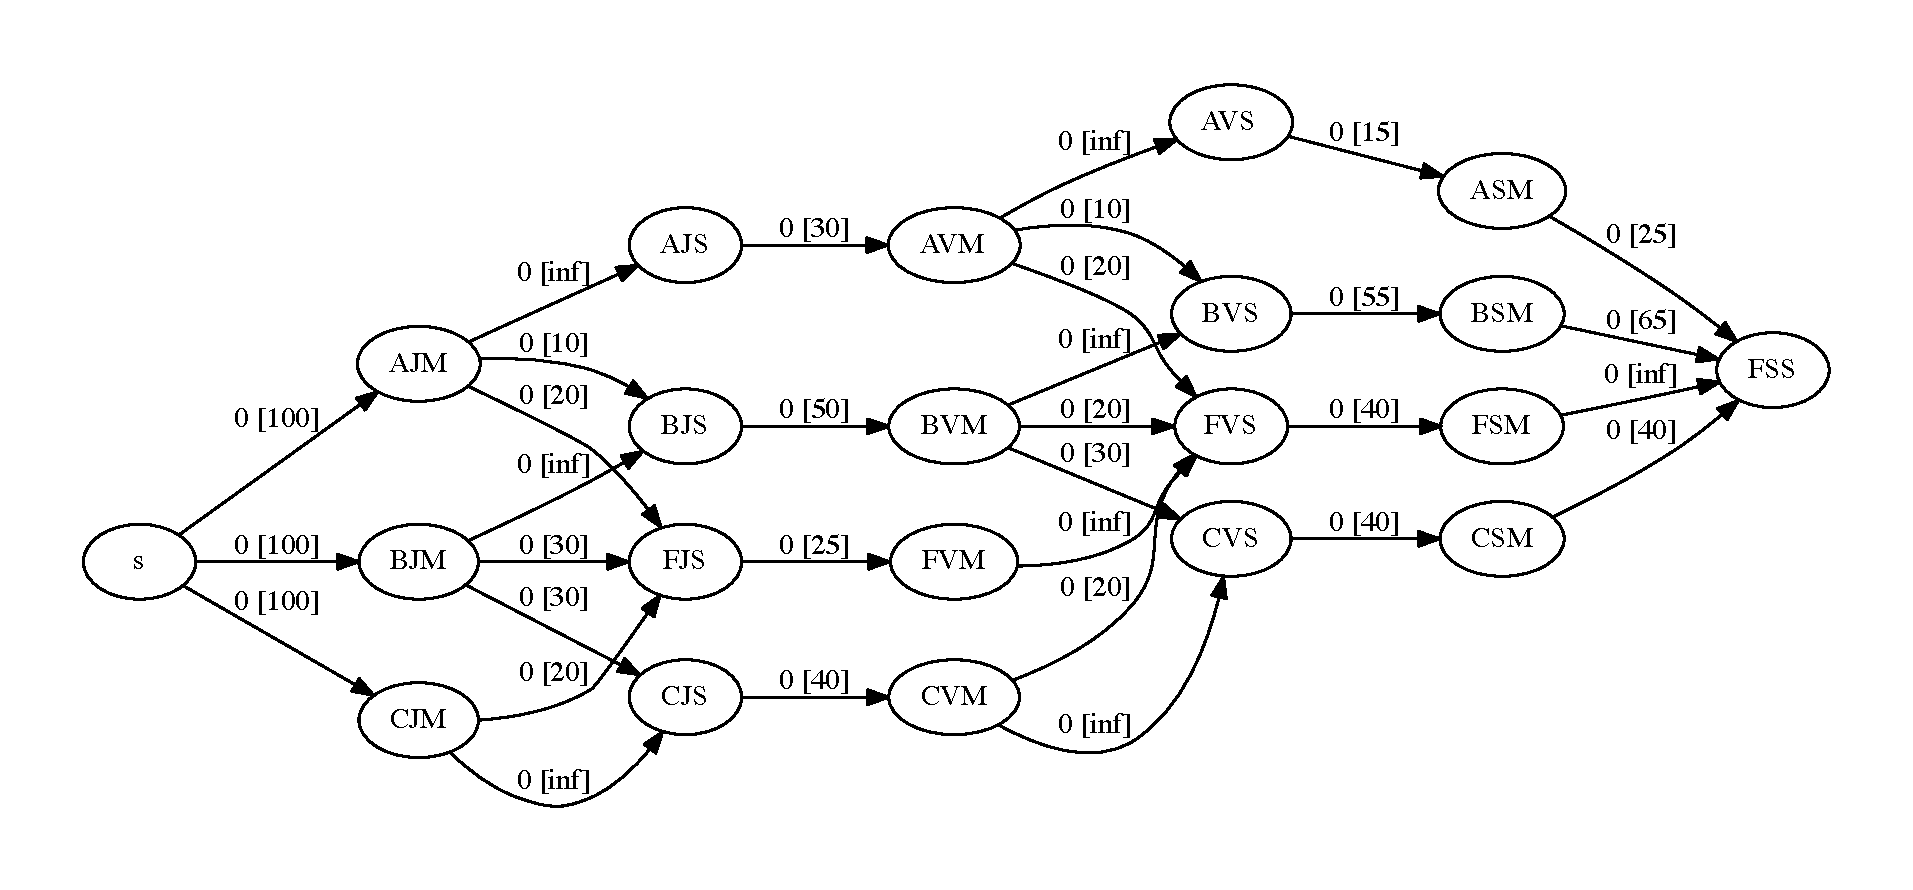
\includegraphics[width=\textwidth]{figs/pass-1.pdf}
	\caption{Graphe initial}
	\label{fig:pass:un}
\end{center}
\end{figure}

Là encore, on peut extraire les chaines augmentantes au fur et mesure en appliquant plus ou moins l'algorithme de marquage.

\begin{enumerate}
\item s-AJM-FJS-FVM-FVS-FSM-FSS : on peut augmenter le flot de 20, voir figure~\ref{fig:pass:deux}
\item s-CJM-CJS-CVM-FVS-FSM-FSS : on peut augmenter le flot de 20, voir figure~\ref{fig:pass:trois}
\item s-BJM-BJS-BVM-BVS-BSM-FSS : on peut augmenter le flot de 50, voir figure~\ref{fig:pass:quatre}
\item s-AJM-AJS-AVM-AVS-ASM-FSS : on peut augmenter le flot de 15, voir figure~\ref{fig:pass:cinq}
\item s-CJM-CJS-CVM-CVS-CSM-FSS : on peut augmenter le flot de 20, voir figure~\ref{fig:pass:six}
\item s-AJM-AJS-AVM-FVS-CVM-CVS-CSM-FSS : on peut augmenter le flot (on a bien ici une \textbf{chaine} augmentante, certains arcs sont utilisés dans le sens puits vers source, le long de l'arc colorié en bleu, on diminue le flot), voir figure~\ref{fig:pass:sept}
\item s-BJM-FJS-FVM-FVS-AVM-BVS-BSM-FSS : on peut augmenter le flot de 5 (toujours en utilisant une \textbf{chaine} augmentante), cf.~\ref{fig:pass:huit}
\end{enumerate}

Il n'existe alors plus de chaine augmentante (figure~\ref{fig:pass:neuf}) : le passage de l'algorithme de marquage ne permettra pas de dépasser le jeudi soir. Cela donne la coupe minimale (en fait la nuit du jeudi au vendredi) pour une valeur de 145. Cela correspond également au flot que nous avons établi et l'algorithme est alors terminé.


\begin{figure}[h]
\begin{center}
	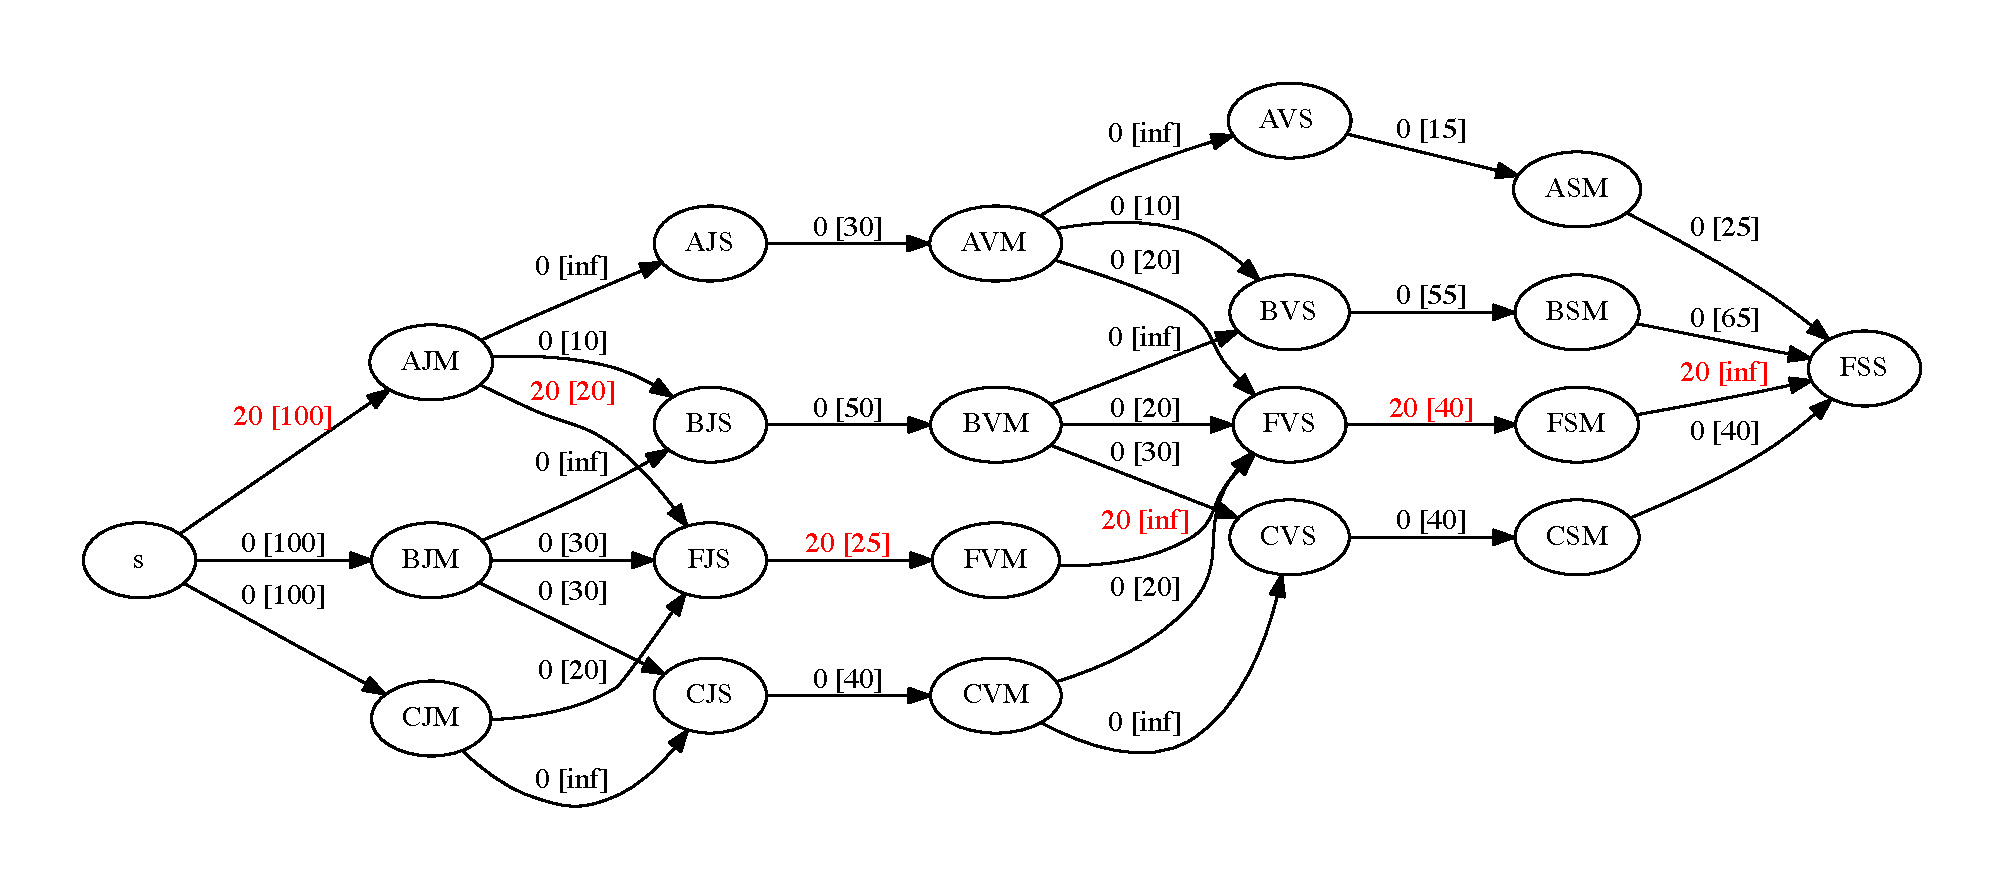
\includegraphics[width=\textwidth]{figs/pass-2.pdf}
	\caption{Première itération}
	\label{fig:pass:deux}
\end{center}
\end{figure}

\begin{figure}[h]
\begin{center}
	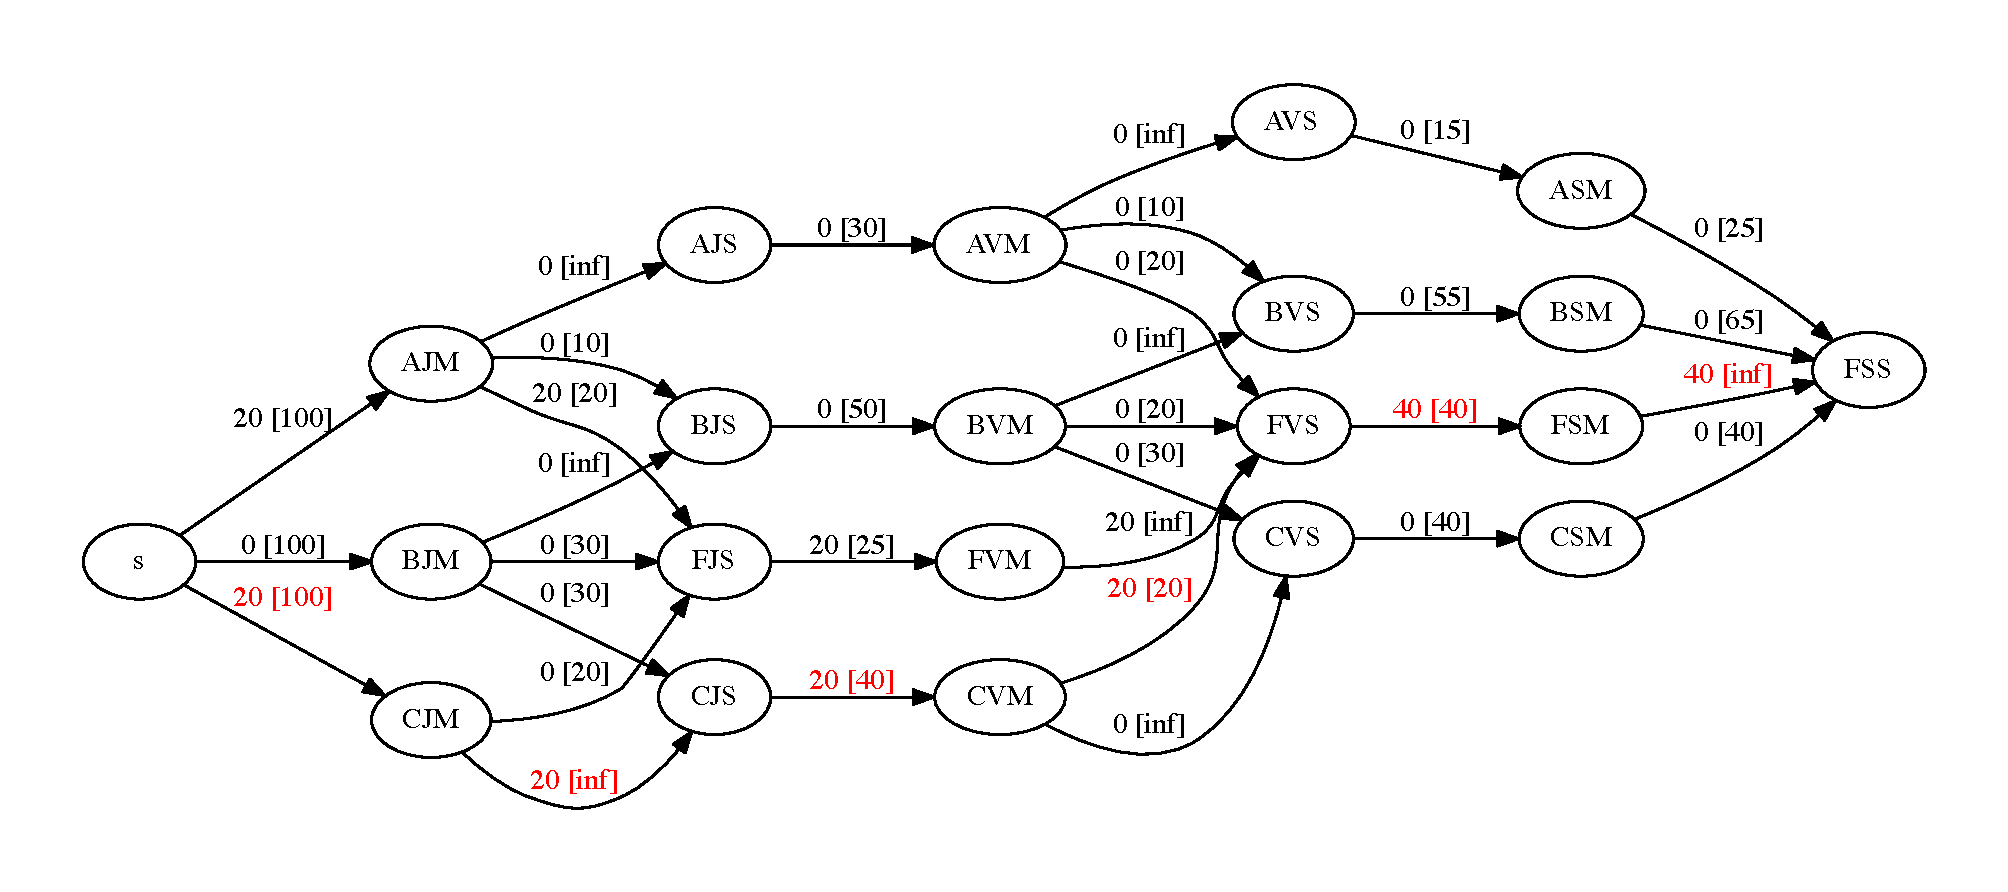
\includegraphics[width=\textwidth]{figs/pass-3.pdf}
	\caption{Seconde itération}
	\label{fig:pass:trois}
\end{center}
\end{figure}

\begin{figure}[h]
\begin{center}
	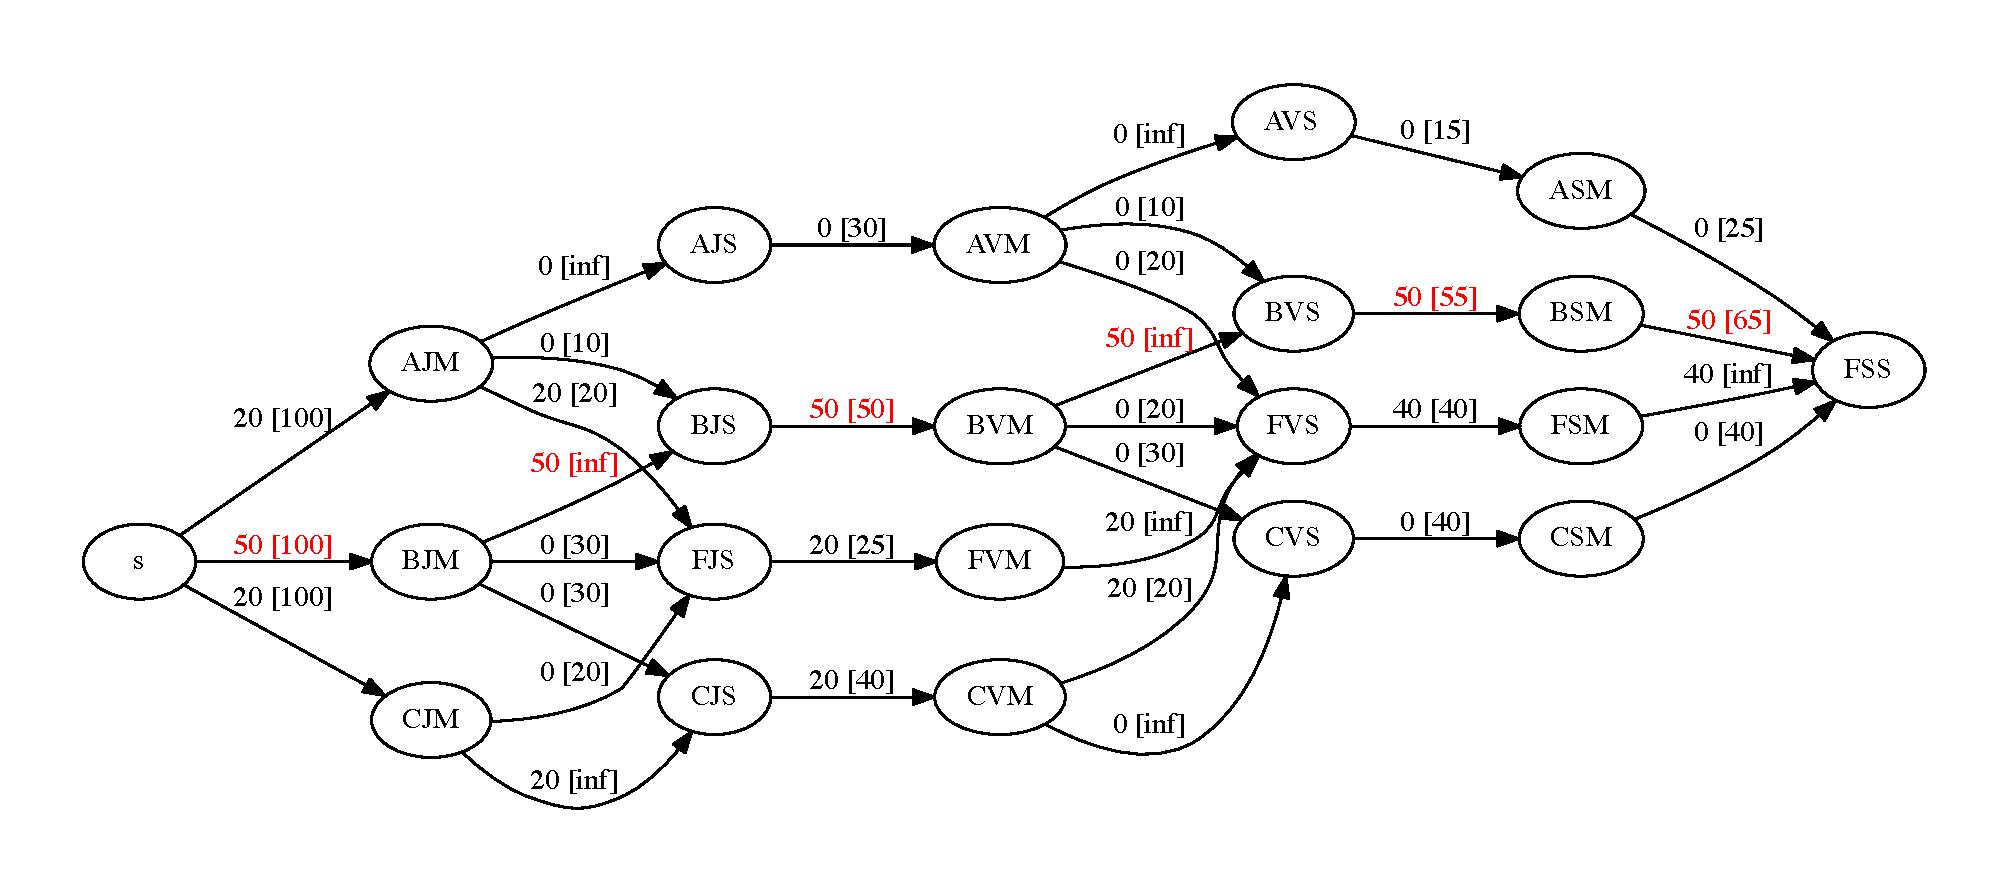
\includegraphics[width=\textwidth]{figs/pass-4.pdf}
	\caption{Troisième itération}
	\label{fig:pass:quatre}
\end{center}
\end{figure}

\begin{figure}[h]
\begin{center}
	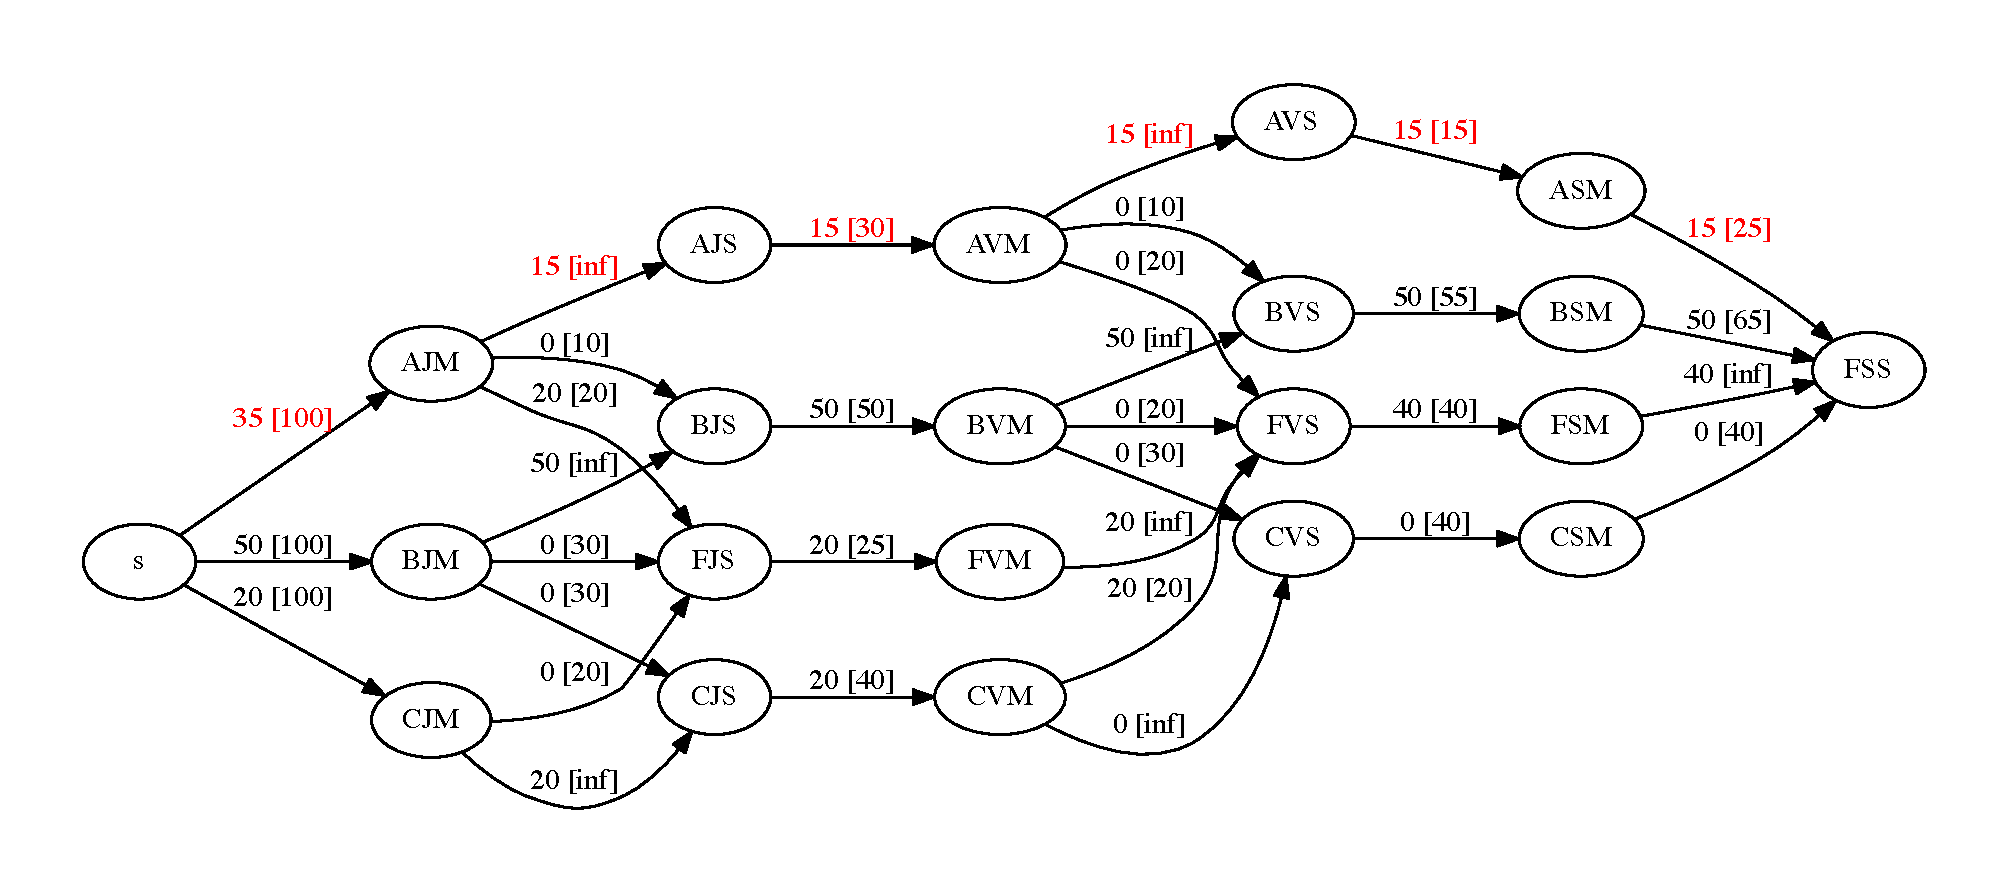
\includegraphics[width=\textwidth]{figs/pass-5.pdf}
	\caption{Quatrième itération}
	\label{fig:pass:cinq}
\end{center}
\end{figure}

\begin{figure}[h]
\begin{center}
	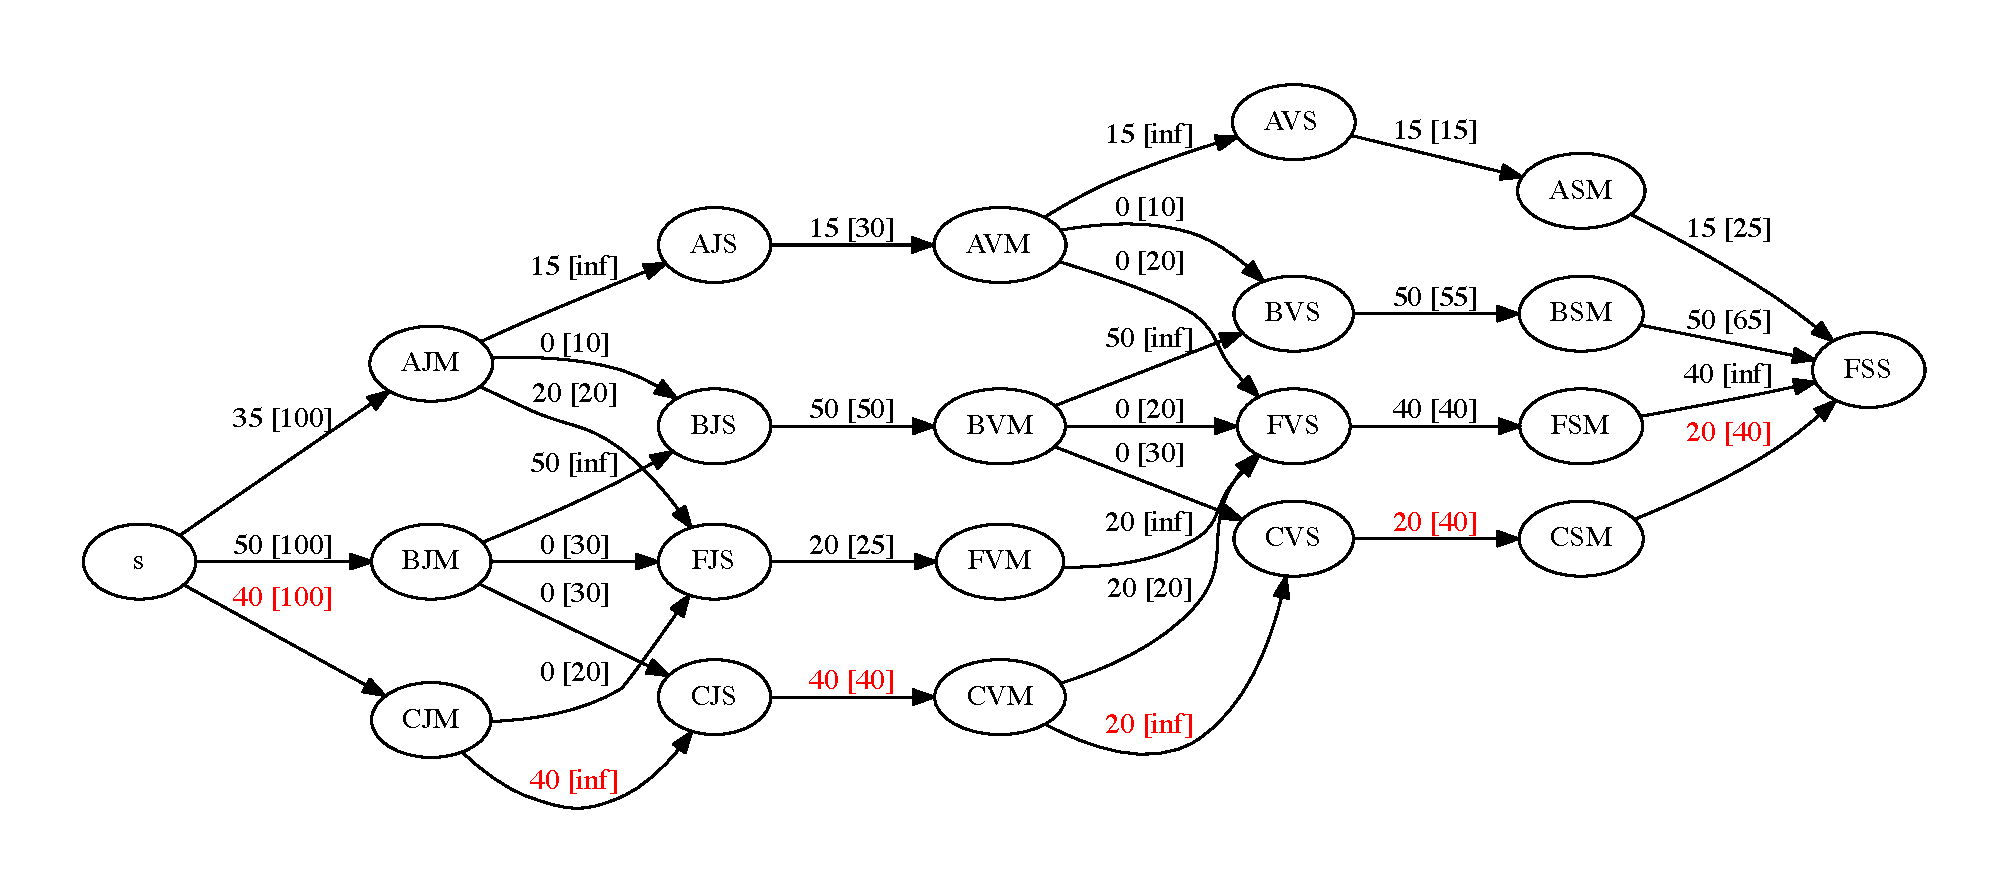
\includegraphics[width=\textwidth]{figs/pass-6.pdf}
	\caption{Cinquième itération}
	\label{fig:pass:six}
\end{center}
\end{figure}

\begin{figure}[h]
\begin{center}
	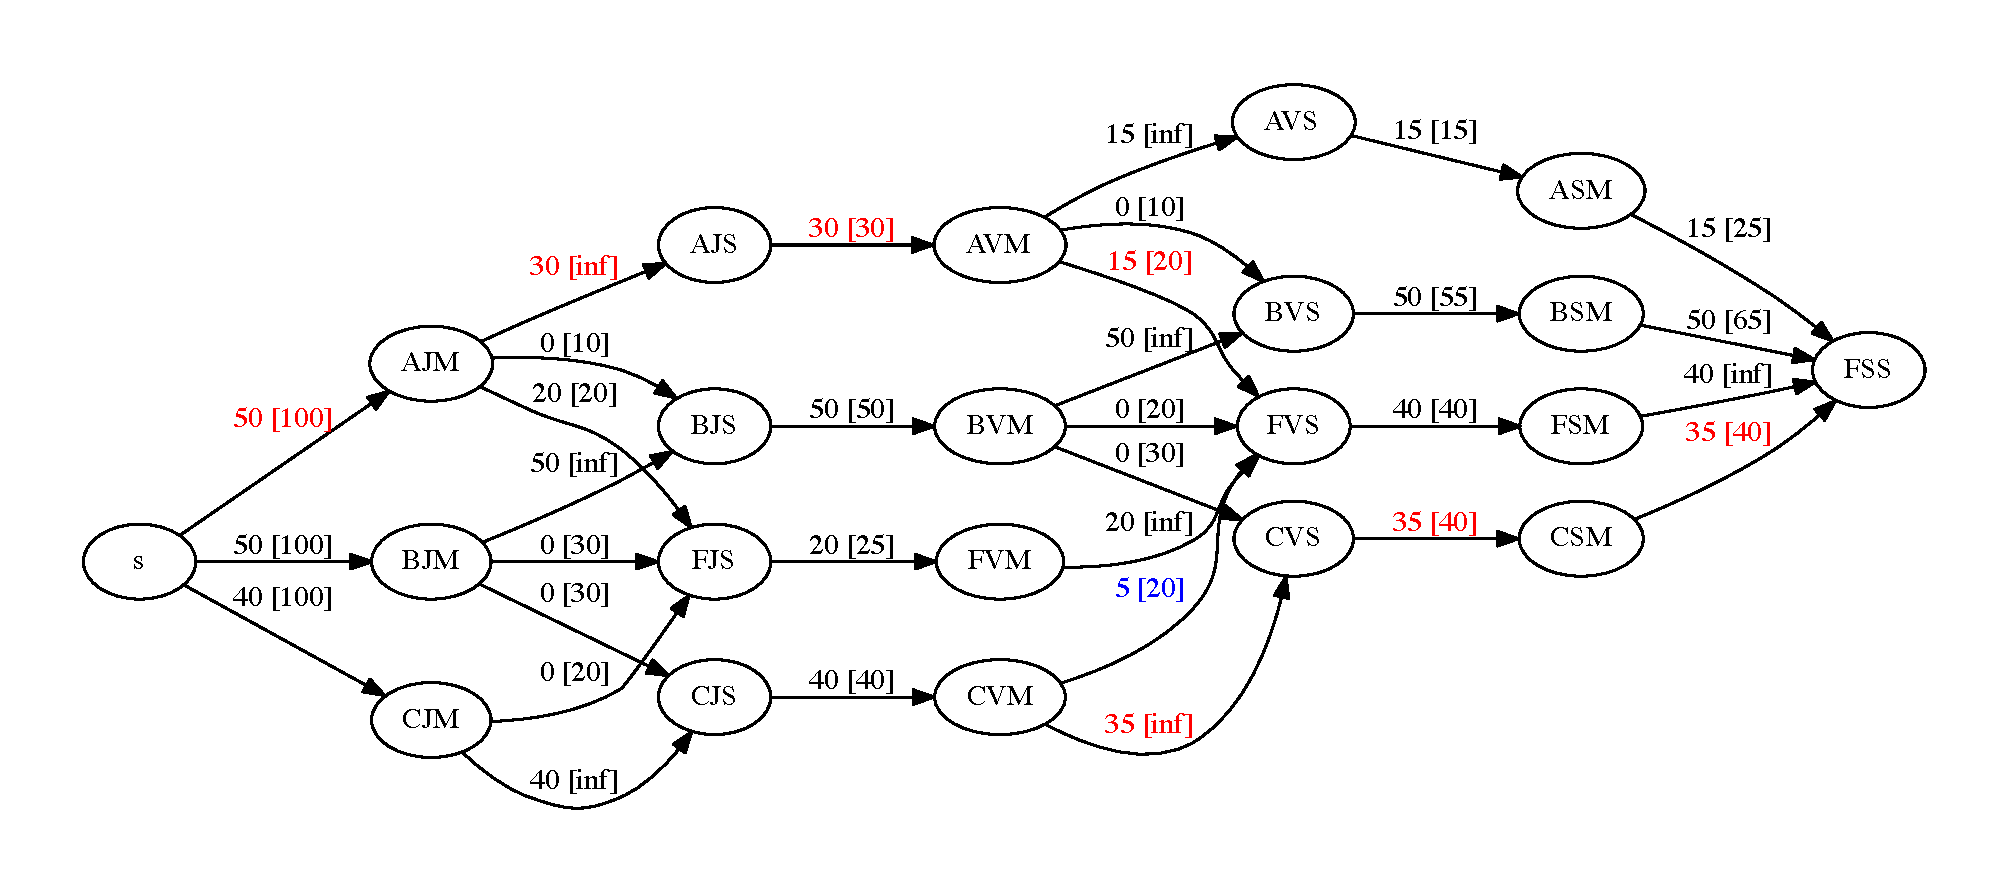
\includegraphics[width=\textwidth]{figs/pass-7.pdf}
	\caption{Sixième itération}
	\label{fig:pass:sept}
\end{center}
\end{figure}

\begin{figure}[h]
\begin{center}
	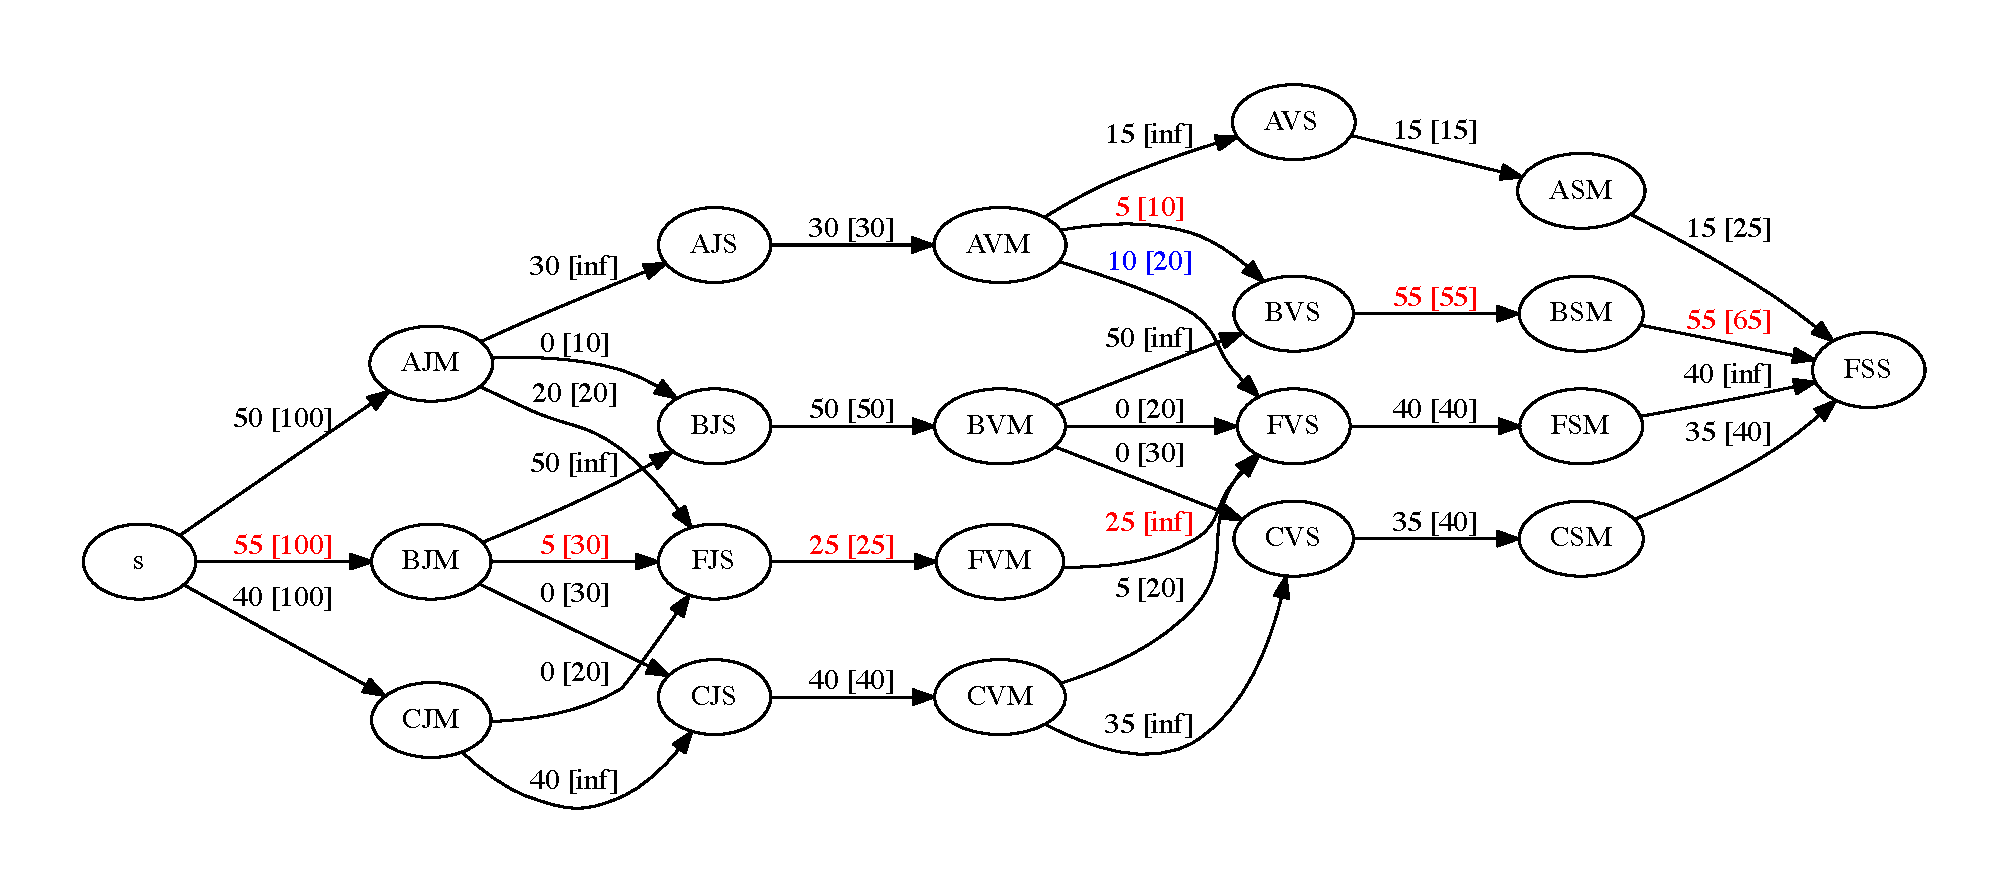
\includegraphics[width=\textwidth]{figs/pass-8.pdf}
	\caption{Septième itération}
	\label{fig:pass:huit}
\end{center}
\end{figure}

\begin{figure}[h]
\begin{center}
	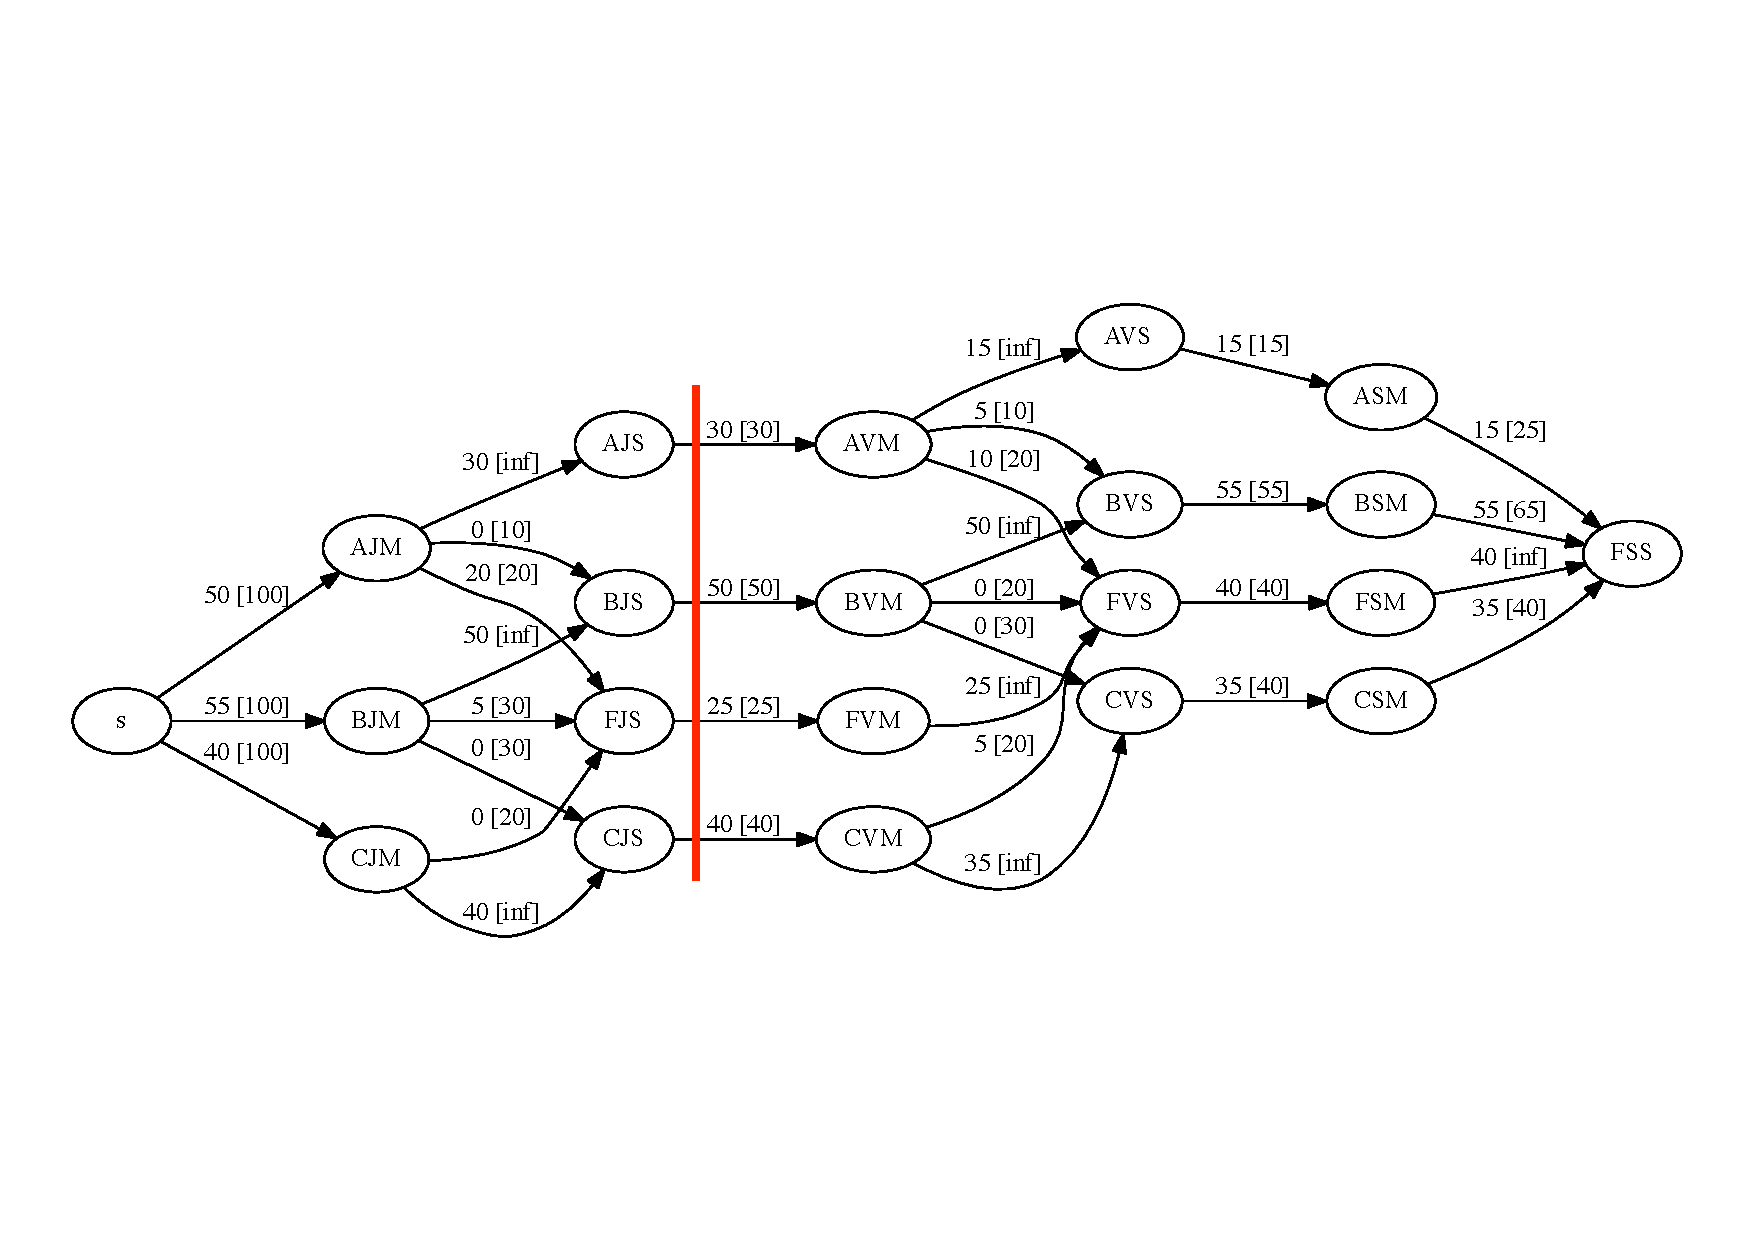
\includegraphics[width=\textwidth]{figs/pass-9.pdf}
	\caption{Flot final et coupe minimale}
	\label{fig:pass:neuf}
\end{center}
\end{figure}

\clearpage
